\documentclass{standalone}

\usepackage{amsmath}
\usepackage{tikz}
\usetikzlibrary{automata, positioning, arrows}

\newcommand{\pushone}{\texttt{\textsc{push}}\textsubscript{\texttt{1}}}
\newcommand{\nonempty}{\textsc{\texttt{nonempty}}}
\newcommand{\tos}{\textsc{\texttt{top}}}
\newcommand{\pop}{\textsc{\texttt{pop}}}
\newcommand{\noop}{\textsc{\texttt{noop}}}

\begin{document}
	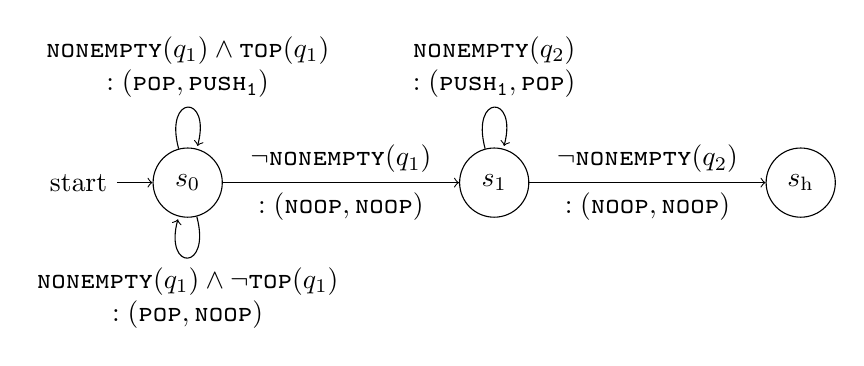
\begin{tikzpicture}[node distance=3cm, ->]
		\node[state, initial] (s0) {$s_0$};
		\node[state, right=of s0] (s1) {$s_1$};
		\node[state, right=of s1] (h){$s_\mathrm{h}$};
		\draw	
			(s0) edge[loop above] node[align=center] {$\nonempty(q_1)\land\tos(q_1)$\\$:(\pop,\pushone)$} (s0) 
			(s0) edge[loop below] node[align=center] {$\nonempty(q_1)\land\lnot\tos(q_1)$\\$:(\pop,\noop)$} (s0)
			(s0) edge[above] node[align=center] {$\lnot\nonempty(q_1)$} (s1)
			(s0) edge[below, draw=none] node[align=center] {$:(\noop,\noop)$} (s1)
			(s1) edge[loop above] node[align=center] {$\nonempty(q_2)$\\$:(\pushone,\pop)$} (s1)
			(s1) edge[above] node[align=center] {$\lnot\nonempty(q_2)$} (h)
			(s1) edge[below, draw=none] node[align=center] {$:(\noop,\noop)$} (h);
	\end{tikzpicture}
\end{document}
